\documentclass[12 pt]{article}

%bibliography
\usepackage[a4paper,width=150mm,top=40mm,bottom=25mm]{geometry}

\usepackage{setspace}
\usepackage{graphicx}

\usepackage{fancyhdr}
\pagestyle{fancy}
\fancyhead{}
\rhead{CHAPTER 2. ANALYSIS OF THE LOCAL GRAPHS}
\fancyfoot{}
\rfoot{\thepage}
\usepackage{multirow}
\usepackage{lscape}

\usepackage[round]{natbib}
\bibliographystyle{abbrvnat}
%\addbibresource{test.bib}

\usepackage{hyperref}
\usepackage{xcolor}
\urlstyle{tt}
\hypersetup{
    colorlinks,
    linkcolor={red!70!black},
    citecolor={blue!70!black},
    urlcolor={magenta!70!black}
}


\title{Accurate sequence variant genotyping in cattle using variation-aware genome graphs}
\author{Danang Crysnanto}
\date{\today}

\begin{document}

\begin{center}
\LARGE\bf{Accurate sequence variant genotyping in cattle using variation-aware genome graphs}
\end{center}

\bigskip
\large{Danang Crysnanto$^{1*}$, Christine Wurmser$^{2}$, Hubert Pausch$^{1}$}

\bigskip 


\normalsize
$^1$ Animal Genomics, ETH Zurich, Zurich, Switzerland. 

$^2$ Chair of Animal Breeding, TU München, Freising, Germany. 

\vspace{2 cm}

\onehalfspacing

In this chapter, I assessed the feasibility of the genome graphs in cattle genome. I assessed \emph{Graphtyper} software for variant genotyping in cattle.  \emph{Graphtyper} performed two round of genotyping. The first is to discover variants from linear
genome. And the second round used the variants discovered in the first round to construct a local genome graph and used it to refine the genotypes. I discovered that \textit{graph genotyping} using \textit{Graphtyper} is highly accurate in cattle and outperform current approaches e.g., \textit{SAMtools, \emph{GATK}} that are based on linear reference. My work is the first to apply \textit{graph genome} for sequence variant genotyping in the livestock genome.  I implemented the graph genotyping pipeline and is now publicly available at \\  
\url{https://github.com/danangcrysnanto/Graph-genotyping-paper-pipelines}. 


\vspace{5 cm}

\bigskip
\large Published in \emph{Genetic Selection Evolution (2019) 51:21.}

\normalsize
\newpage

%First document. This is a simple example, with no 
%extra parameters or packages included.
%What I can do \emph{test this} \textbf{abcdf}.
%Test citation \citep{rice2020}.
%Second approach is \cite{Rosen2020}
\begin{abstract}   
\onehalfspacing

\textbf{Background}: The genotyping of sequence variants typically involves as a first step the alignment of sequencing reads to a linear reference genome. 
Because a linear reference genome represents only a small fraction of sequence variation within a species, reference allele bias may occur at highly polymorphic or diverged regions of the genome. Graph-based methods facilitate to compare sequencing reads to a variation-aware genome graph that incorporates a collection of non-redundant DNA sequences that segregate within a species. We compared accuracy and sensitivity of graph-based sequence variant genotyping using the \emph{Graphtyper} software to two widely used methods, i.e., \emph{GATK} and \emph{SAMtools}, that rely on linear reference genomes using whole-genomes sequencing data of 49 Original Braunvieh cattle.   
\medskip

\textbf{Results}: We discovered 21,140,196, 20,262,913 and 20,668,459 polymorphic sites using \emph{GATK}, \emph{Graphtyper}, and \emph{SAMtools}, respectively. Comparisons between sequence variant and microarray-derived genotypes showed that \emph{Graphtyper} outperformed both \emph{GATK} and \emph{SAMtools} in terms of genotype concordance, non-reference sensitivity, and non-reference discrepancy. The sequence variant genotypes that were obtained using \emph{Graphtyper} had the lowest number of mendelian inconsistencies for both SNPs and indels in nine sire-son pairs with sequence data. Genotype phasing and imputation using the \emph{Beagle} software improved the quality of the sequence variant genotypes for all tools evaluated particularly for animals that have been sequenced at low coverage. Following imputation, the concordance between sequence- and microarray-derived genotypes was almost identical for the three methods evaluated, i.e., 99.32, 99.46, and 99.24 \% for \emph{GATK}, \emph{Graphtyper}, and \emph{SAMtools}, respectively. Variant filtration based on commonly used criteria improved the genotype concordance slightly but it also decreased sensitivity. \emph{Graphtyper} required considerably more computing resources than  \emph{SAMtools} but it required less than \emph{GATK}.   
\medskip  

\textbf{Conclusions}: Sequence variant genotyping using \emph{Graphtyper} is accurate, sensitive and computationally feasible in cattle. Graph-based methods enable sequence variant genotyping from variation-aware reference genomes that may incorporate cohort-specific sequence variants which is not possible with the current implementations of state-of-the-art methods that rely on linear reference genomes. 

\medskip
\textbf{Keywords}: Sequence variant genotyping, Genome graph, Variation-aware graph, cattle, Whole-genome sequencing

\end{abstract}

\newpage

\section{Introduction}

\doublespacing 

The sequencing of important ancestors of many cattle breeds revealed millions of sequence variants that are polymorphic in dairy and beef populations \citep{Hoff2017,Stothard2015,Boussaha2016,Jansen2013}. In order to compile an exhaustive catalog of polymorphic sites that segregate in Bos taurus, the 1000 Bull Genomes consortium was established \citep{Daetwyler2014,Hayes2019}. 
The 1000 Bull Genomes Project imputation reference panel facilitates to infer sequence variant genotypes for large cohorts of genotyped animals thus enabling genomic investigations at nucleotide resolution \citep{Daetwyler2014,Pausch2017,Bouwman2018,Raymond2018}.

Sequence variant discovery and genotyping typically involves two steps that are carried out successively \citep{nielsen2011genotype,guo2014three,goodwin2016coming,pfeifer2017next}: first, raw sequencing data are generated, trimmed and filtered to remove adapter sequences and bases with low sequencing quality, respectively, and aligned towards a linear reference genome using, e.g., \emph{Bowtie} \citep{langmead2012fast} or the Burrows-Wheeler Alignment (\emph{BWA}) software \citep{li2009fast}. The aligned reads are subsequently compared to the nucleotide sequence of a reference genome in order to discover and genotype polymorphic sites using, e.g., \emph{SAMtools} \citep{li2009sequence} or the Genome Analysis Toolkit (\emph{GATK}) \citep{mckenna2010genome,van2013fastq,poplin2018scaling}. Variant discovery may be performed either in single- or multi-sample mode. The accuracy (i.e., ability to correctly genotype sequence variants) and sensitivity (i.e., ability to detect true sequence variants) of sequence variant discovery is higher using multi-sample than single-sample approaches particularly when the sequencing depth is low \citep{liu2013variant,cheng2014assessing,baes2014evaluation,kumar2014evaluation,depristo2011framework}. However, the genotyping of sequence variants from multiple samples simultaneously is a computationally intensive task, particularly when the sequenced cohort is large and diverse and had been sequenced at high coverage \citep{poplin2018scaling}. The multi-sample sequence variant genotyping approach that has been implemented in the \emph{SAMtools} software has to be restarted for the entire cohort once new samples are added. \emph{GATK} implements two different approaches to multi-sample variant discovery, i.e., the UnifiedGenotyper and HaplotypeCaller modules, with the latter relying on intermediate files in gVCF format that include probabilistic data on variant and non-variant sites for each sequenced sample. Applying the HaplotypeCaller module allows for separating variant discovery within samples from the estimation of genotype likelihoods across samples. Once new samples are added to an existing cohort, only the latter needs to be performed for the entire cohort, thus enabling computationally efficient parallelization of sequence variant genotyping in a large number of samples.  

Genome graph-based methods consider non-linear reference sequences for variant discovery \citep{rakocevic2019fast,eggertsson2017graphtyper,novak2017genome,garrison2018variation,sibbesen2018accurate}. A variation-aware genome graph may incorporate distinct (population-specific) reference sequences and known sequence variants. Recently, the \emph{Graphtyper} software has been developed in order to facilitate sequence variant discovery from a genome graph that has been constructed and iteratively augmented using variation of the sequenced cohort \citep{eggertsson2017graphtyper}. So far, sequence variant genotyping using variation-aware genome graphs has not been evaluated in cattle.

An unbiased evaluation of the accuracy and sensitivity of sequence variant genotyping is possible when high confidence sequence variants and genotypes are accessible that were detected using genotyping technologies and algorithms different from the ones to be evaluated \citep{li2018synthetic}. For species where such a resource is not available, the accuracy of sequence variant genotyping may be evaluated by comparing sequence variant to microarray-derived genotypes (e.g., \citep{Jansen2013,depristo2011framework}). Due to the ascertainment bias in SNP chip data, this comparison may overestimate the accuracy of sequence variant discovery particularly at variants that are either rare or located in less-accessible genomic regions \citep{li2014toward,malomane2018efficiency}.

In this study, we compare sequence variant discovery and genotyping from a variation-aware genome graph using \emph{Graphtyper} to two state-of-the-art methods (\emph{GATK}, \emph{SAMtools}) that rely on linear reference genomes in 49 Original Braunvieh cattle. We compare sequence variant to microarray-derived genotypes in order to assess accuracy and sensitivity of sequence variant genotyping for each of the three methods evaluated.

\section{Methods}

\paragraph{Selection of animals} 

We selected 49 Original Braunvieh (OB) bulls that were either frequently used in artificial insemination or explained a large fraction of the genetic diversity of the active breeding population. Semen straws of the bulls were purchased from an artificial insemination center and DNA was prepared following standard DNA extraction protocols.

\paragraph{Sequencing data pre-processing}

All samples were sequenced on either an Illumina HiSeq 2500 (30 animals) or an Illumina HiSeq 4000 (19 animals) sequencer using 150 bp paired-end sequencing libraries with insert sizes ranging from 400 to 450 bp. Quality control (removal of adapter sequences and bases with low quality) of the raw sequencing data was caried out using the \emph{fastp} software (version 0.19.4) with default parameters \citep{chen2018fastp}. The filtered reads were mapped to the UMD3.1 version of the bovine reference genome \citep{zimin2009whole} using \emph{BWA mem} (version 0.7.12) \citep{li2009fast} with option-M to mark shorter split hits as secondary alignments, default parameters were applied in all other steps. Optical and PCR duplicates were marked using \emph{Samblaster} (version 0.1.24) \citep{faust2014samblaster}. The output of \emph{Samblaster} was converted into BAM format using \emph{SAMtools view} (version 1.3) \citep{li2009sequence}, and subsequently coordinate-sorted using \emph{Sambamba} (version 0.6.6) \citep{tarasov2015sambamba}. We used the \emph{GATK} (version 3.8) \emph{RealignerTargetCreator} and \emph{IndelRealigner} modules to realign reads around indels. The realigned BAM files served as input for \emph{GATK} base quality score recalibration using 102,092,638 unique positions from the Illumina BovineHD SNP chip and Bovine dbSNP version 150, as known variants. The \emph{mosdepth} software (version 0.2.2) \citep{pedersen2018mosdepth} was used to extract the number of reads that covered a genomic position.

\paragraph{Sequence variant discovery}

We followed the best practice guidelines recommended for variant discovery and genotyping using \emph{GATK} (version 4.0.6) with default parameters for all commands \citep{mckenna2010genome,vander2018best,depristo2011framework}. First, genotype likelihoods were calculated separately for each sequenced animal using \emph{GATK HaplotypeCaller} \citep{vander2018best}, which resulted in files in gVCF (genomic Variant Call Format) format for each sample \citep{danecek2011variant}. The gVCF files from the 49 samples were consolidated using \emph{GATK} GenomicsDBImport. Subsequently, \emph{GATK GenotypeGVCFs} was applied to genotype polymorphic sequence variants for all samples simultaneously.

\emph{Graphtyper} (version 1.3) was run in a multi-sample mode as recommended in Eggertsson et al. \citep{eggertsson2017graphtyper}. Because the original implementation of \emph{Graphtyper} is limited to the analysis of the human chromosome complement, we cloned the \emph{Graphtyper GitHub} repository (\url{https://github.com/DecodeGenetics/graphtyper}), modified the source code to allow analysis of the cattle chromosome complement, and compiled the program from the modified source code (see Additional file 1). The \emph{Graphtyper} workflow consisted of four steps that were executed successively. First, sequence variants were identified from the read alignments that were produced using \emph{BWA mem} (see above). Second, these cohort-specific variants were used to augment the UMD3.1 reference genome and construct the variation-aware genome graph. Third, the sequencing reads were locally realigned against the variation-aware graph. A clean variation graph was produced by removing unobserved haplotypes paths from the raw graph. In the final step, genotypes were identified from the realigned reads in the clean graph. The  \emph{Graphtyper} pipeline was run in segments of 1 million bp and whenever the program failed to genotype variants for a particular segment either because it ran out of memory or exceeded the allocated runtime of 12 h, the interval was subdivided into smaller segments (10 kb).

Our implementation of  \emph{SAMtools}mpileup (version 1.8) \citep{li2011statistical} was run in a multi-sample mode to calculate genotype likelihoods from the aligned reads for all samples simultaneously. The parameters -E and -t were used to recalculate (and apply) base alignment quality and produce per-sample genotype annotations, respectively. Next, the estimated genotype likelihoods were converted into genotypes using BCFtools call using the -v and -m flags to output variable sites only, and permit sites to have more than two alternative alleles, respectively.

We implemented all pipelines using Snakemake (version 5.2.0) [46]. The scripts for the pipelines are available via \emph{Github} repository \\
\url{https://github.com/danangcrysnanto/Graph-genotyping-paper-pipelines}

\paragraph{Sequence variant filtering and genotype refinement}

The \emph{GATK VariantFiltration} module was used to parse and filter the raw VCF files. Quality control on the raw sequencing variants and genotypes was applied according to guidelines that were recommended for each variant caller. Variants that were identified using \emph{GATK} were retained if they met the following criteria: QualByDepth (QD) $>$ 2.0, FisherStrand $>$ 60.0, RMSMappingQuality (MQ) $>$ 40.0, MappingQualityRankSumTest (MQRankSum) $>$ 12.5, ReadPosRankSumTest (ReadPosRankSum) $>$ -8.0, SOR $<$ 3.0 (SNPs) and QD $>$ 2.0, FS $<$ 200.0, ReadPosRankSum $>$ 20.0, SOR $<$ 10.0 (indels). For the variants identified using \emph{SAMtools}, the thresholds that have been applied in the 1000 Bull Genomes project \citep{Daetwyler2014} were considered to remove variants with indication of low quality. Variants were retained if they met the following criteria: QUAL $>$ 20, MQ $>$ 30, ReadDepth (DP) $>$ 10, DP $<$ median(DP) $+$ 3 $*$ mean(DP).   
Moreover, SNPs were removed from the data if they had the same positions as the starting position of an indel. The output of \emph{Graphtyper} was filtered so that it included only variants that met criteria recommeded by Eggertsson et al. \citep{eggertsson2017graphtyper}: ABHet $<$ 0.0 $|$ ABHet $>$ 0.33, ABHom $<$ 0.0 $|$ ABHom $>$ 0.97, MaxAASR $>$ 0.4, and MQ $>$ 30. 

We used \emph{Beagle} (version 4.1) \citep{browning2016genotype} to improve the raw sequence variant genotype quality and impute missing genotypes. The genotype likelihood (\emph{gl}) mode of \emph{Beagle} was applied to infer missing and modify existing genotypes based on the phred-scaled likelihoods (\emph{PL}) of all other non-missing genotypes of the 49 Original Braunvieh animals in our study.

\paragraph{Evaluation of sequence variant genotyping}

To ensure consistent variant representation across the different sequence variant genotyping methods evaluated, we applied the \emph{vt normalize} software (version 0.5) \citep{tan2015unified}. Normalized variants are parsimonious (i.e., represented by as few nucleotides as possible) and left aligned \citep{tan2015unified}. The number of variants detected and transition to transversion (Ti/Tv) ratios were calculated using \emph{vt peek} \citep{tan2015unified} and \emph{BCFtools stats} \citep{li2011statistical}. The intersection of variants that were common to the evaluated tools was calculated and visualized using \emph{BCFtools isec} \citep{li2011statistical} and the UpSet R package \citep{conway2017upsetr}, respectively.

Mendelian inconsistencies were calculated as the proportion of variants showing opposing homozygous genotypes in nine parent–offspring pairs that were included in the 49 sequenced animals. For this comparison, we considered only the sites for which the genotypes of both sire and son were not missing.

All    49    sequenced    cattle    were    also    genotyped    using  either  the  Illumina  BovineHD  (N  =  29)  or  the  BovineSNP50 (N = 20) Bead chip that comprise 777,962 and  54,001  SNPs,  respectively.  The  average  genotyping  rate  at  autosomal  SNPs  was  98.91\%.  In  order  to  assess  the  quality  of  sequence  variant  genotyping,  the  genotypes  detected  by  the  different  variant  calling  methods  were compared  to  the  array-called  genotypes  in  terms  of  genotype  concordance,  non-reference  sensitivity  and  non-reference discrepancy \citep{depristo2011framework,linderman2014analytical}, and for more details on  the  metrics  (see  Additional  file 2).  Non-parametric  Kruskal–Wallis   tests   followed   by   pairwise   Wilcoxon   signed-rank tests were applied to determine if any of the three  metrics  differed  significantly  between  the  three  tools evaluated.


\paragraph{Computing environment and statistical analysis}

All computations were performed on the ETH Zurich Leonhard Open Cluster with access to multiple nodes equipped with 18 cores Intel Xeon E5-2697v4 processors (base frequency rated at 2.3 GHz) and 128 GB of random-access memory. Unless otherwise stated, the R (version 3.3.3) software environment \citep{team2013r} was used for statistical analyses and ggplot2 (version 3.0.0) \citep{wickham2016ggplot2} was used for data visualisation.

\section{Results}

Following  quality  control  (removal  of  adapter  sequences  and  low-quality  bases),  we  aligned  more  than  13  billion  paired-end  reads  (2 × 125  and  2 × 150  bp)  from  49  Original  Braunvieh  cattle  to  the  UMD3.1  assembly  of  the  bovine  genome.  On  average,  98.44\%  (91.06–99.59\%)  of  the  reads  mapped  to  the  reference  genome  and  4.26\%  (2.0–10.91\%) of these were flagged as duplicates and not considered for further analyses. Sequencing depth ranged from  6.00  to  37.78  with  an  average  depth  per  animal  of  12.75  and  was  above  12-fold  for  31  samples.  Although  the  realignment  of  sequencing  reads  around  indels  is  no  longer  required  when  sequence  variants  are  genotyped  using  the  latest  version  of  \emph{GATK}  (v  4),  it  is  still  recommended  to  improve  the  genotyping  of  indels  by  using \emph{SAMtools}. To ensure a fair comparison of the three tools evaluated,  we  realigned  the  reads  around  indels  on  all  BAM files and used the re-aligned files as a starting point for our comparisons (Fig. \ref{fig:loca}). The sequencing read data of 49 cattle were deposited at European Nucleotide Archive (ENA) (\url{http://www.ebi.ac.uk/ena})  under  primary  accession PRJEB28191. \\

\begin{figure}[h]
    \centering
    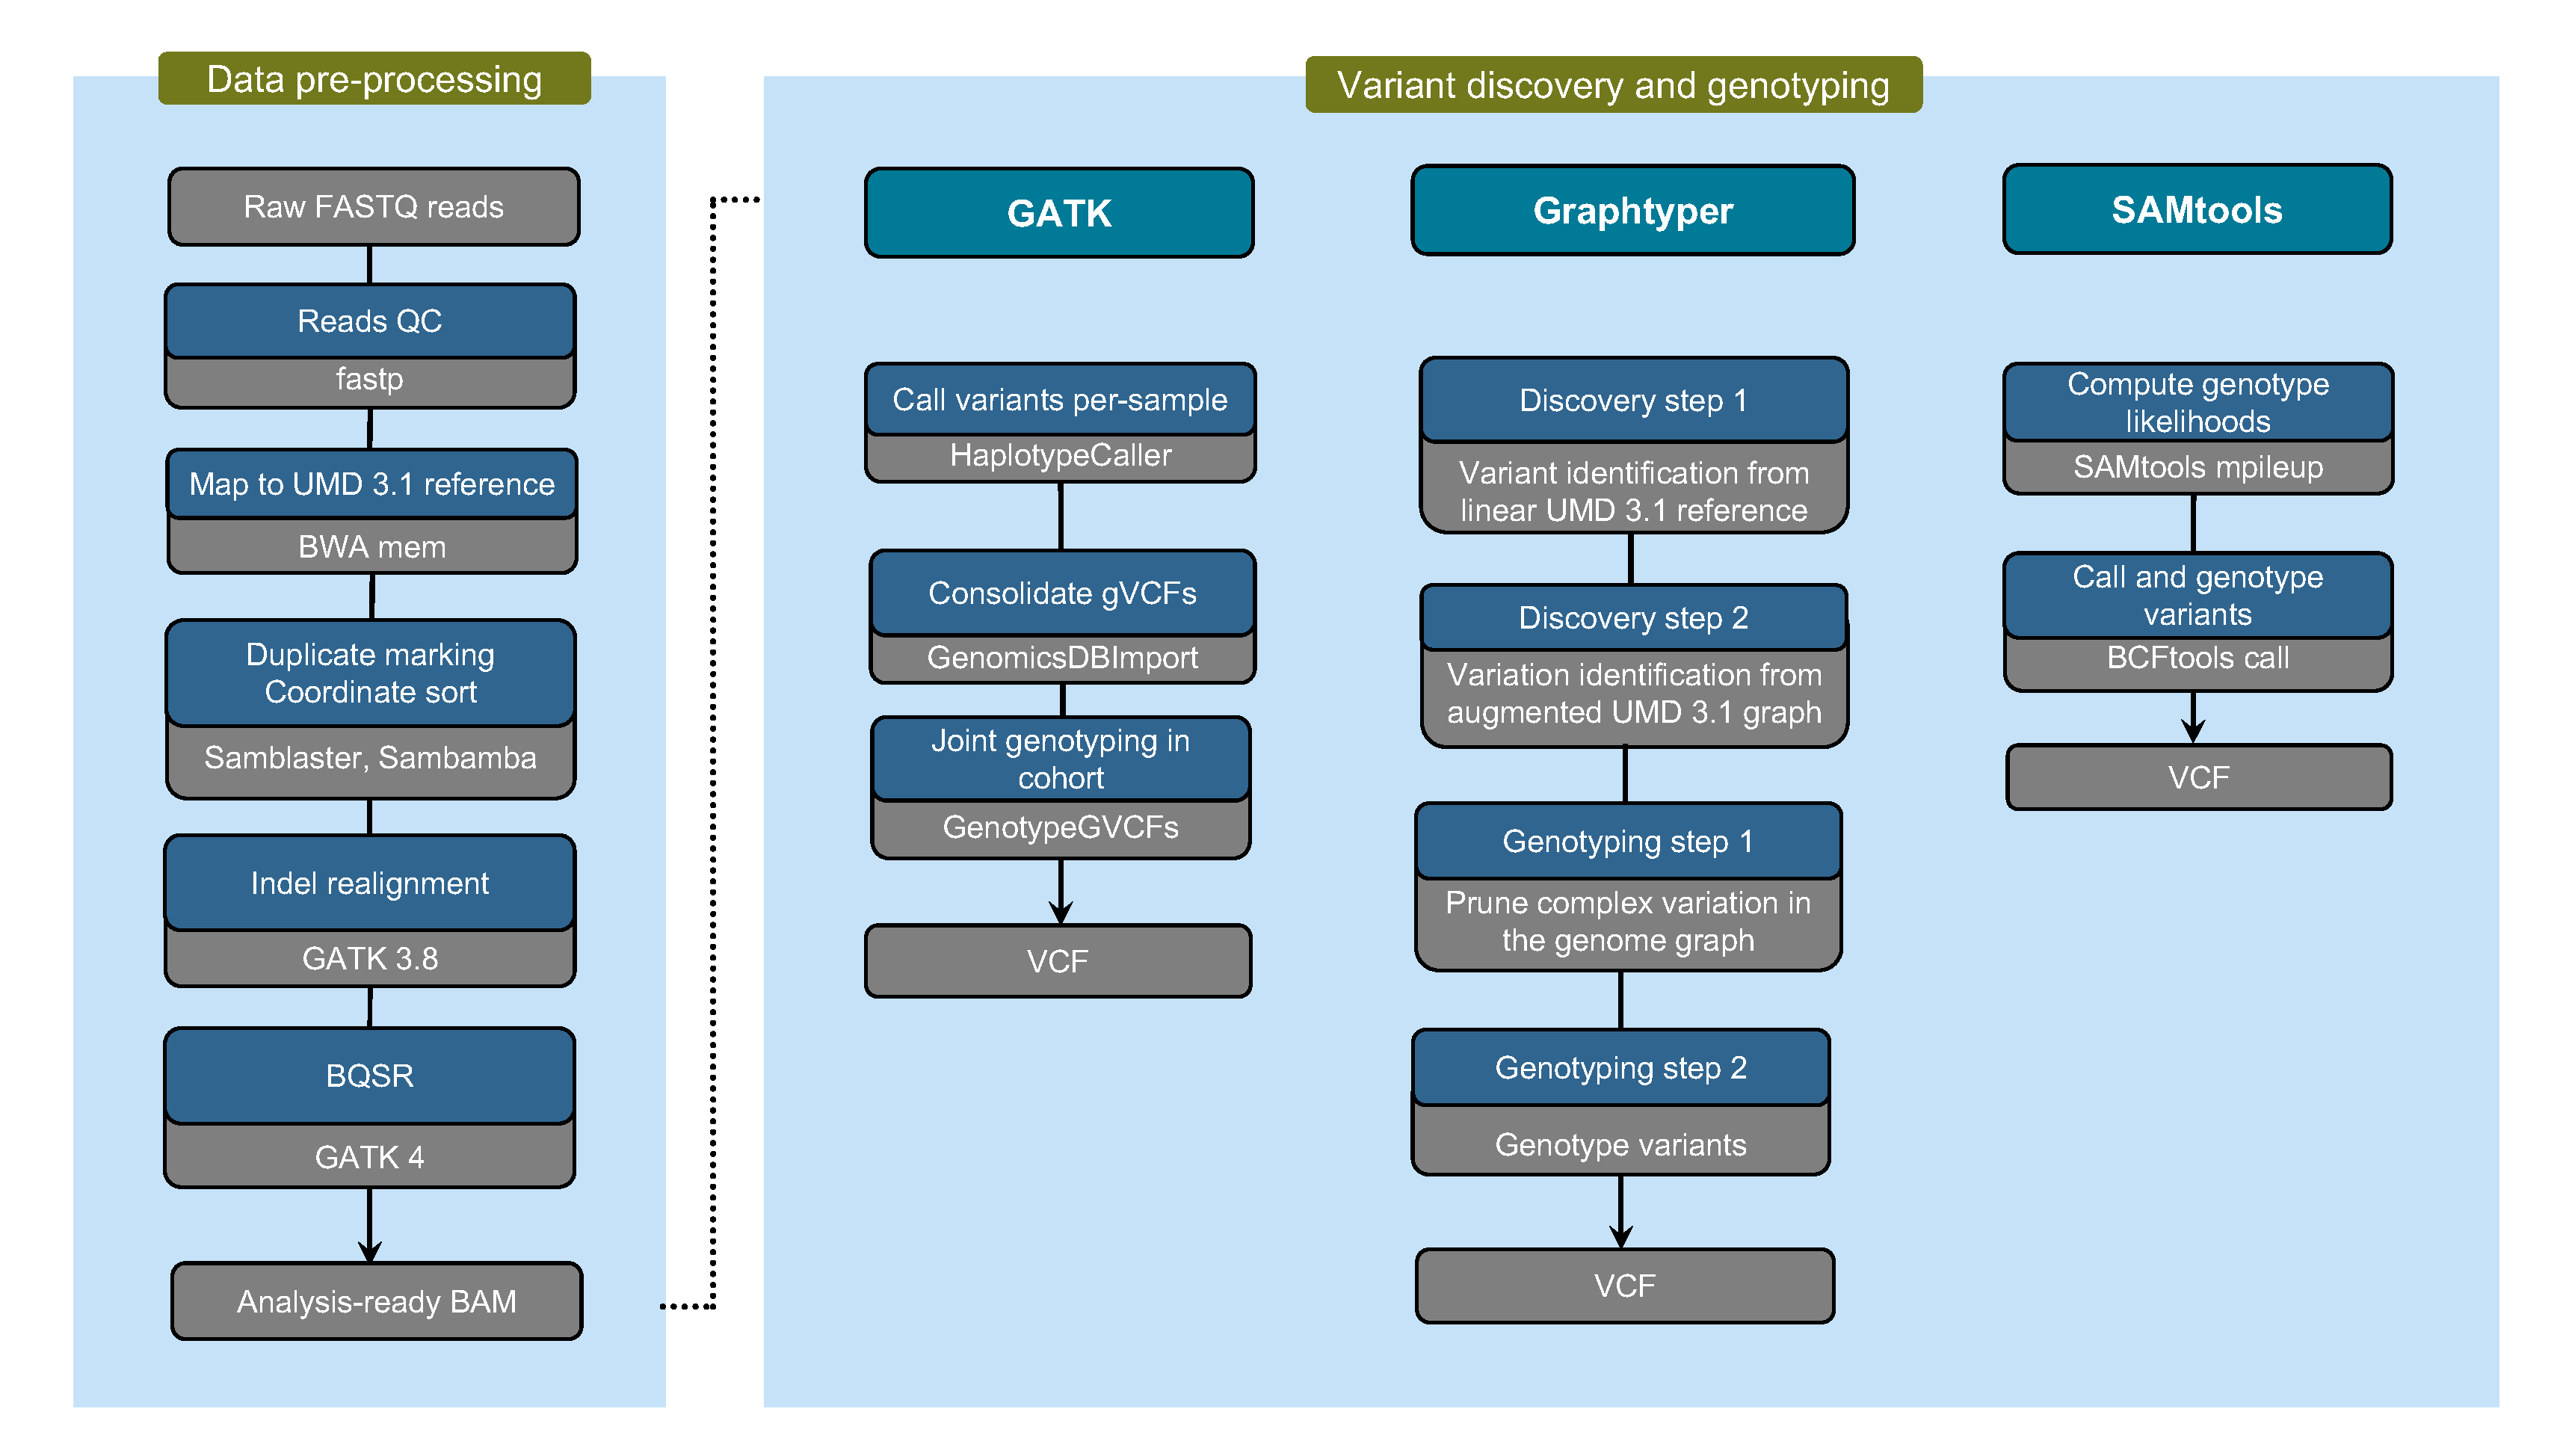
\includegraphics[width=\textwidth]{figure/paper1/main_figure/Figure1.pdf}
    \caption[Pipeline methods]{\textbf{Schematic representation of the three sequence variant discovery and genotyping methods evaluated.} \\
    \small{According to the best practice recommendations for sequence variant discovery using \emph{GATK}, the VQSR module should be applied to distinguish between true and false positive variants. Because this approach requires a truth set of variants, which is not (publicly) available for cattle, the VQSR module was not considered in our evaluation}}
    \label{fig:loca}
\end{figure}

\subsection*{Sequence variant discovery and genotyping}

Polymorphic  sites  (SNPs,  indels)  were  discovered  and  genotyped in the 49 animals using either \emph{GATK} (version 4), \emph{Graphtyper}  (version  1.3)  or  \emph{SAMtools}  (version  1.8).  All software programs were run using default parameters and  workflow  descriptions  for  variant  discovery  (Fig. \ref{fig:loca} and  also  see  Methods).  Only  autosomal  sequence  variants  were  considered  to  evaluate  the  accuracy  and  sen-sitivity  of  sequence  variant  genotyping.  Because  variant  filtering has a strong impact on the accuracy and sensitivity of sequence variant genotyping \citep{carson2014effective,jun2015efficient}, we evaluated both  the  raw  variants  that  were  detected  using  default  parameters  for  variant  discovery  (Fig. \ref{fig:loca})  and  variants  that  remained  after  applying  filtering  criteria  that  are  commonly  used  but  may  differ  slightly  between  different software tools. Note that \emph{GATK} was run by using the suggested filtering parameters, when application of Variant Quality Score Recalibration (VQSR) is not possible.

Using default parameters for variant discovery for each of the software programs evaluated, 21,140,196, 20,262,913, and 20,668,459 polymorphic sites were discovered using \emph{GATK},  \emph{Graphtyper} and SAMtools, respectively (Table \ref{tab:varcount}). The vast majority (86.79, 89.42 and 85.11\%) of the detected variants were biallelic SNPs. Of the 18,594,182, 18,120,724 and 17,592,038 SNPs detected using \emph{GATK},  \emph{Graphtyper} and SAMtools, respectively, 7.46, 8.31 and 5.02\% were novel, i.e., they were not among the 102,091,847 polymorphic sites of the most recent version (150) of the Bovine dbSNP database. The Ti/Tv ratio of the detected SNPs was equal to 2.09, 2.07 and 2.05 using \emph{GATK},  \emph{Graphtyper} and SAMtools, respectively. Using \emph{GATK} revealed four times more multiallelic SNPs (246,220) than either  \emph{SAMtools}or  \emph{Graphtyper}.



\begin{landscape}
\begin{table}
    \vspace{10mm} 
    \centering
    \caption{\textbf{Number of different types of autosomal sequence variants} detected in 49 Original Braunvieh cattle using three sequence variant genotyping methods (Full) and subsequent variant filtration based on commonly used criteria (Filtered)}
    \vspace{10mm}
    \begin{tabular}{|l|l|l|l|l|l|l|} 
    \cline{2-7}
    \multicolumn{1}{l|}{} & \multicolumn{3}{c|}{\multirow{2}{*}{Full}}                                      & \multicolumn{3}{c|}{\multirow{2}{*}{Filtered}}                                   \\
    \multicolumn{1}{l|}{} & \multicolumn{3}{l|}{}                                                           & \multicolumn{3}{l|}{}                                                            \\ 
    \cline{2-7}
    \multicolumn{1}{l|}{} & \multirow{2}{*}{GATK} & \multirow{2}{*}{Graphtyper} & \multirow{2}{*}{SAMtools} & \multirow{2}{*}{GATK} & \multirow{2}{*}{Graphtyper} & \multirow{2}{*}{SAMtools}  \\ 
    \cline{1-1}
                          &                       &                             &                           &                       &                             &                            \\ 
    \hline
    Variants              & 21,140,196            & 20,262,913                  & 20,668,459                & 19,761,679            & 17,679,155                  & 18,871,549                 \\ 
    \hline
    \multicolumn{7}{|l|}{}                                                                                                                                                                     \\ 
    \hline
    SNPs                  & 18,594,182            & 18,120,724                  & 17,592,038                & 17,248,593            & 15,777,446                  & 16,272,917                 \\ 
    \hline
    Not in dbSNP          & 1,387,781             & 1,505,586                   & 882,575                   & 867,838               & 564,326                     & 570,901                    \\ 
    \hline
    Biallelic             & 18,347,962            & 18,053,396                  & 17,528,249                & 17,111,806            & 15,730,153                  & 16,218,714                 \\ 
    \hline
    Multi-allelic         & 246,220               & 67,328                      & 63,789                    & 136,787               & 47,293                      & 54,203                     \\ 
    \hline
    Ti/Tv ratio           & 2.09                  & 2.07                        & 2.05                      & 2.17                  & 2.18                        & 2.16                       \\ 
    \hline
    SNP array (\%)        &                       &                             &                           &                       &                             &                            \\ 
    \hline
    BovineHD              & 99.46                 & 99.61                       & 99.32                     & 99.21                 & 98.79                       & 98.85                      \\ 
    \hline
    Bovine SNP50          & 99.14                 & 99.26                       & 99.12                     & 98.91                 & 98.87                       & 98.9                       \\ 
    \hline
    \multicolumn{7}{|l|}{}                                                                                                                                                                     \\ 
    \hline
    Indels                & 2,478,489             & 2,044,585                   & 3,076,421                 & 2,445,766             & 1,826,808                   & 2,598,632                  \\ 
    \hline
    Not in dbSNP          & 663,831               & 596,137                     & 1,279,162                 & 639,219               & 456,752                     & 979,291                    \\ 
    \hline
    Biallelic             & 2,166,352             & 1,753,391                   & 2,704,413                 & 2,133,840             & 1,571,195                   & 2,310,386                  \\ 
    \hline
    Multi-allelic         & 312,137               & 291,194                     & 372,008                   & 311,926               & 255,613                     & 288,246                    \\ 
    \hline
    Insertion/Deletion    & 0.88                  & 0.88                        & 1                         & 0.88                  & 0.88                        & 0.99                       \\ 
    \hline
    Complex variation     & 67,525                & 97,604                      & 0                         & 67,320                & 74,901                      & 0                          \\
    \hline
    \end{tabular}
    \label{tab:varcount}
    \end{table}
\end{landscape}

\newpage

We identified 2,478,489, 2,044,585, and 3,076,421 indels using GATK, Graphtyper, and SAMtools, respectively, and 26.78\%, 29.15\%, and 41.75\% of them were novel. SAMtools revealed the largest number and highest proportion (14.9\%) of indels. Between 12 and 14\% of the detected indels were multiallelic. While Graphtyper and GATK identified more (12\%) deletions than insertions, the proportions were almost the same using SAMtools.

On average, each Original Braunvieh cattle carried between 7 and 8 million variants that differed from the UMD3.1 reference genome. Of these, between 2.4 and 2.6 million SNPs were homozygous for the alternate allele, between 3.8 and 4.7 million SNPs were heterozygous and between 0.7 and 1 million were indels (Table \ref{tab:varhet}).

An intersection of 15,901,526 biallelic SNPs was common to all sequence-variant discovery tools evaluated (Fig. 2a), i.e., between 85.51 and 90.39\% of the detected SNPs of each tool, and 466,029 (2.93\%, Ti/Tv: 1.81) of them were novel, i.e., they were not present in dbSNP 150. The Ti/Tv-ratio of the common SNPs was 2.22. SAMtools had the largest number of SNPs in common with the other two tools (90.39\%). The number of private SNPs, i.e., SNPs that were detected by one but not the other tools was largest for GATK and smallest for Graphtyper.


\newpage

\begin{landscape}
\begin{table}
    \centering
    \caption{\textbf{Average number of autosomal variants} identified per animal using three sequence variant genotyping methods}
    \vspace{10 mm}
    \begin{tabular}{|l|l|l|l|l|l|l|} 
    \cline{2-7}
    \multicolumn{1}{l|}{}  & \multicolumn{3}{c|}{\multirow{2}{*}{Full}}              & \multicolumn{3}{c|}{\multirow{2}{*}{Filtered}}           \\
    \multicolumn{1}{l|}{}  & \multicolumn{3}{l|}{}                                   & \multicolumn{3}{l|}{}                                    \\ 
    \cline{2-7}
    \multicolumn{1}{l|}{}  & \textit{GATK} & \textit{Graphtyper} & \textit{SAMtools} & \textit{GATK} & \textit{Graphtype}r & \textit{SAMtools}  \\ 
    \hline
    Total biallelic SNPs   & 6,324,455     & 7,384,058           & 6,617,948         & 6,105,674     & 6,533,711           & 6,564,229          \\ 
    \hline
    Heterozygous           & 3,890,351     & 4,758,297           & 4,187,882         & 3,744,336     & 4,074,011           & 4,147,033          \\ 
    \hline
    Homozygous ALT         & 2,434,104     & 2,625,761           & 2,430,066         & 2,361,338     & 2,459,700           & 2,417,196          \\ 
    \hline
    Ti/Tv                  & 2.17          & 2.13                & 2.11              & 2.2           & 2.14                & 2.13               \\ 
    \hline
    Total biallelic indels & 693,697       & 767,261             & 1,007,420         & 691,765       & 697,637             & 960,218            \\ 
    \hline
    Heterozygous           & 390,495 s      & 441,172             & 616,981           & 388,622       & 391,856             & 593,417            \\ 
    \hline
    Homozygous ALT         & 303,202       & 326,089             & 390,439           & 303,143       & 305,781             & 366,801            \\ 
    \hline
    Singletons             & 49,166        & 23,406              & 32,810            & 41,408        & 17,999              & 32,398             \\
    \hline
    \end{tabular}
    \label{tab:varhet}
    \end{table}
    \singlespacing
    \small{The number of variants is presented for the three tools evaluated before (Full) and after (Filtered) applying recommended filters to identify and exclude low quality variants}
\end{landscape}

\newpage

\begin{figure}[h]
    \centering
    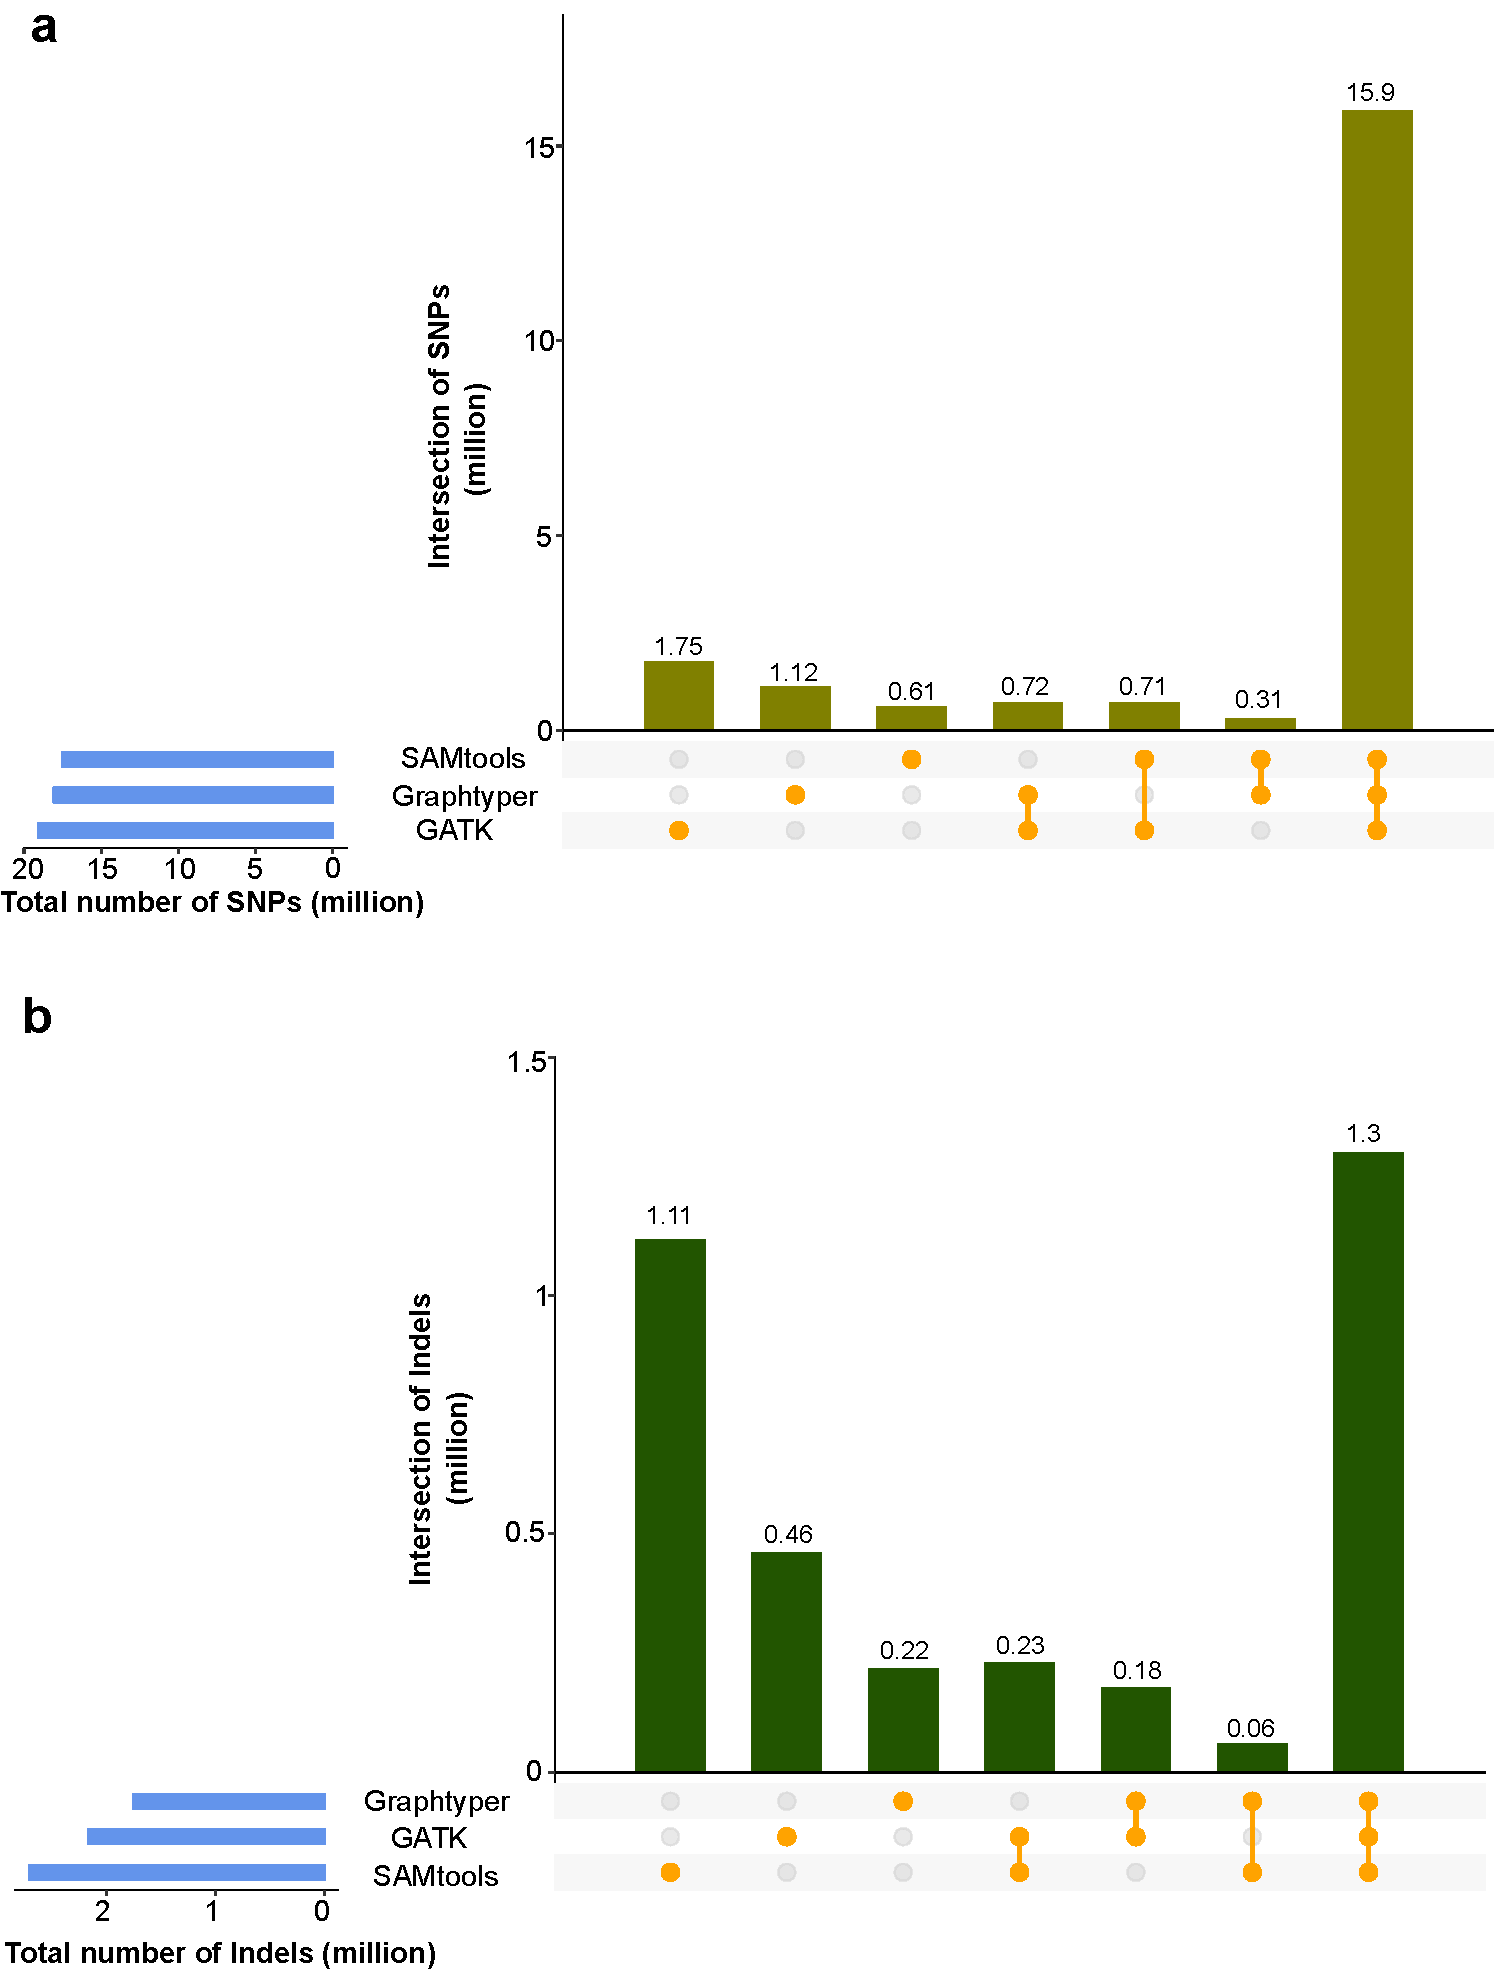
\includegraphics[width=\textwidth]{figure/paper1/main_figure/Figure2.pdf}
    \caption{Number of biallelic SNPs (\textbf{a}) and indels (\textbf{b}) identified in 49 Original Braunvieh cattle using three sequence variant genotyping methods. Blue horizontal bars represent the total number of sites discovered for each method. Vertical bars indicate private and common variants detected by the methods evaluated}
    \label{fig:varoverlap}
\end{figure}

\singlespacing
\footnotesize

\bibliography{combined_ref}

\end{document}